% fig_arch_wide (full width, 7.16 in): the detector with its training items and one block opened up.
% Sources: results/research/retouch_unified_20260929/train_ru5.py (RUCLIP5, RUData5, loss_fn incl. Addendum 46),
% train_ru_clip.py (RUCLIP: LoRALinear on q_proj/k_proj/v_proj/out_proj of every encoder layer, r=16),
% docs/paper_v2/main_v6b.tex Sec. Method (triplets, footprint M = dilate(1[|x-x0|_inf > 6])).
\documentclass[tikz,border=1.5pt]{standalone}
% Shared visual language of the TikZ figures (fig_arch, fig_system, fig_protocol, fig_exposure, fig_explain_layers).
% Colours are the palette of docs/paper_v2/figstyle.py: house blue for our model, Okabe-Ito green / vermillion for correct /
% error, light fills by stage type (network, code, language model, check, fallback, input/output), thin dark arrows.
% Text: TeX Gyre Heros (Helvetica metrics), 7 pt body; tensor shapes in DejaVu Sans Mono 5.5 pt.
\usepackage{fontspec}
\setsansfont{texgyreheros}[Extension=.otf,UprightFont=*-regular,BoldFont=*-bold,ItalicFont=*-italic,BoldItalicFont=*-bolditalic]
\setmonofont{DejaVuSansMono}[Path=/usr/share/fonts/truetype/dejavu/,Extension=.ttf,BoldFont=*-Bold,Scale=0.92]
\renewcommand{\familydefault}{\sfdefault}
\usepackage{amsmath}
\usepackage[italic]{mathastext}
\usetikzlibrary{positioning,arrows.meta,fit,backgrounds,calc,shapes.misc,decorations.pathreplacing}

% ---- palette (figstyle.py) -----------------------------------------------------------------------------------------
\definecolor{ink}{HTML}{222222}
\definecolor{muted}{HTML}{6B6B6B}
\definecolor{gridc}{HTML}{E5E5E5}
\definecolor{ours}{HTML}{0F4D92}     % house blue: our model, trainable parts
\definecolor{oursarm}{HTML}{5B9BD5}
\definecolor{okc}{HTML}{009E73}      % genuine / correct
\definecolor{errc}{HTML}{D55E00}     % forged / error
\definecolor{amber}{HTML}{C98A00}    % language model (deck palette)
\definecolor{plum}{HTML}{A8538A}     % checks
\definecolor{truth}{HTML}{56B4E9}    % ground-truth footprint
\definecolor{hilite}{HTML}{FFD700}
% light fills by stage type
\definecolor{fNet}{HTML}{E2EBF6}
\definecolor{fCode}{HTML}{DFF2EA}
\definecolor{fLLM}{HTML}{FCEFD6}
\definecolor{fChk}{HTML}{F6E6F0}
\definecolor{fFall}{HTML}{FBE4D8}
\definecolor{fIO}{HTML}{F4F4F4}

\newcommand{\bodyfont}{\fontsize{7}{8.2}\selectfont}
\newcommand{\smallfont}{\fontsize{6.2}{7.2}\selectfont}
\newcommand{\shp}[1]{{\fontsize{5.6}{6.4}\selectfont\ttfamily\color{muted}#1}}   % tensor-shape annotation
\newcommand{\hd}[1]{{\bfseries #1}}

\tikzset{
  every picture/.style={line width=0.5pt, font=\bodyfont, >={Stealth[length=3.4pt,width=2.8pt]}},
  stage/.style={rounded corners=2.2pt, draw=#1!75!black, line width=0.5pt, align=center, inner sep=2.6pt},
  net/.style={stage=ours, fill=fNet},
  code/.style={stage=okc, fill=fCode},
  llm/.style={stage=amber, fill=fLLM},
  chk/.style={stage=plum, fill=fChk},
  fall/.style={stage=errc, fill=fFall},
  io/.style={stage=muted, fill=fIO},
  plain/.style={rounded corners=2.2pt, draw=ink!55, fill=white, align=center, inner sep=2.6pt},
  flow/.style={->, draw=ink, line width=0.55pt},
  tflow/.style={->, draw=ink, line width=0.55pt, dash pattern=on 2.2pt off 1.4pt},   % training-time only
  errflow/.style={->, draw=errc, line width=0.6pt},
  okflow/.style={->, draw=okc, line width=0.6pt},
  thumb/.style={inner sep=0pt, draw=muted, line width=0.35pt},
  lbl/.style={font=\smallfont, text=ink, align=center, inner sep=1pt},
  note/.style={font=\smallfont, text=muted, align=center, inner sep=1pt},
  badge/.style={rounded corners=5pt, draw=#1, fill=white, line width=0.5pt, font=\smallfont\bfseries, text=#1, inner xsep=3pt, inner ysep=1.6pt},
}

\newcommand{\vdotsdraw}[1]{\foreach \d in {-0.08,0,0.08}{\fill[muted] ($(#1)+(0,\d)$) circle (0.5pt);}}
\newcommand{\panel}[2]{\node[anchor=north west, font=\bodyfont\bfseries, text=ink, inner sep=0pt] at (#1) {#2};}
\newcommand{\trainitem}[6]{% y, file, title, description, colour, name
  \node[thumb, draw=#5, line width=0.7pt] (t#6) at (0.5,#1) {\includegraphics[width=0.9cm]{img/#2.png}};
  \node[anchor=north west, align=left, inner sep=0pt, font=\smallfont\bfseries] (lab#6) at (1.05,#1+0.43) {#3};
  \node[anchor=north west, align=left, inner sep=0pt, font=\smallfont, text=muted] at ([yshift=-1.5pt]lab#6.south west) {#4};}
\begin{document}
\begin{tikzpicture}[x=1cm,y=1cm]
% ================================================================ (a) training items
\panel{0,2.55}{a\;\; training items}
\trainitem{1.6}{x0}{genuine $x_0$}{untreated frame}{okc}{g}
\trainitem{0.4}{x0_smooth}{beautified}{landmark or skin op,\\[-1pt]colour filter or grading}{okc}{b}
\trainitem{-0.8}{x}{forged}{self-blend, FF++ fake\\[-1pt]or part edit; beautified\\[-1pt]on top w.p. 0.5}{errc}{f}
\node[thumb, draw=ours, dash pattern=on 1.6pt off 1pt, line width=0.6pt] (txs) at (0.5,-2.15) {
\includegraphics[width=0.9cm]{img/xs.png}};
\node[anchor=north west, align=left, inner sep=0pt, font=\smallfont\bfseries, text=ours] (labs) at (1.05,-1.72) {$x_s$ of every item};
\node[anchor=north west, align=left, inner sep=0pt, font=\smallfont, text=muted] at ([yshift=-1.5pt]labs.south west) {skin-smoothed copy,\\[-1pt]same operator for\\[-1pt]both classes};
\draw[decorate, decoration={brace, amplitude=3pt}, draw=muted] (3.22,2.05) -- (3.22,-1.25);

% ================================================================ (b) backbone with one block opened
\panel{3.6,2.55}{b\;\; backbone}
\node[net, minimum width=2.35cm, minimum height=4.3cm] (vit) at (4.95,0.0) {};
\node[anchor=north, font=\smallfont\bfseries, text=ours] at ([yshift=-1.5pt]vit.north) {CLIP ViT-L/14};
\node[anchor=north, note] at ([yshift=-9pt]vit.north) {frozen weights};
\foreach \y/\t in {1.25/1, 0.8/2, -0.15/24}{
  \node[draw=ink!40, fill=white, rounded corners=1.2pt, minimum width=2.05cm, minimum height=0.36cm] (b\t) at (4.95,\y) {};
  \node[font=\fontsize{5.6}{6}\selectfont, text=muted, inner sep=0pt] at (4.12,\y) {\t};
  \foreach \k/\n in {0/q,1/k,2/v,3/o}{
    \node[draw=ours, fill=fNet, line width=0.45pt, minimum size=0.25cm, inner sep=0pt, font=\fontsize{5.4}{6}\selectfont\ttfamily]
      at (4.4+\k*0.28,\y) {\n};}
  \node[draw=ink!35, fill=fIO, rounded corners=0.8pt, minimum width=0.48cm, minimum height=0.25cm, inner sep=0pt,
        font=\fontsize{5.2}{6}\selectfont, text=muted] at (5.66,\y) {MLP};
}
\vdotsdraw{4.95,0.33}
\node[anchor=north, font=\smallfont, text=muted] at (4.95,-0.4) {24 blocks};
\node[anchor=south, font=\fontsize{5.9}{6.8}\selectfont, text=muted, inner sep=1pt] (prm) at ([yshift=2pt]vit.south) {3.2\,M of 306\,M trained};
\node[anchor=south, align=center, font=\fontsize{5.9}{6.8}\selectfont, inner sep=1pt, text=ours] at (prm.north)
  {LoRA, rank 16,\\[-0.5pt]on q, k, v, o};
\draw[flow] (3.35,0.4) -- node[above, inner sep=1pt]{\shp{x}} (vit.west |- 0,0.4);
\draw[tflow] (txs.south) -- (0.5,-2.95) -| (4.3,0 |- vit.south);
\node[anchor=north west, note, inner sep=1pt] at (1.2,-2.95) {same weights};

% opened block (a zoom, not on the data path)
\node[draw=ink!50, rounded corners=2pt, fill=white, minimum width=2.9cm, minimum height=2.95cm] (blk) at (7.95,-0.55) {};
\draw[densely dotted, draw=ink!50] (b24.north east) -- (blk.north west);
\draw[densely dotted, draw=ink!50] (b24.south east) -- (blk.south west);
\node[anchor=north west, font=\smallfont\bfseries, text=ink, inner sep=0pt] at ([xshift=3pt,yshift=-3pt]blk.north west) {one block};
\begin{scope}[every node/.style={font=\smallfont, inner sep=1.1pt}]
  \node[draw=ink!35, fill=fIO, rounded corners=1pt, minimum width=0.95cm] (ln1) at (7.15,0.45) {LN};
  \node[draw=ink!45, fill=fIO, rounded corners=1pt, minimum width=1.05cm, align=center] (W) at (7.15,-0.15) {$W$ \shp{1024²}};
  \node[draw=ours, fill=fNet, rounded corners=1pt, minimum width=0.45cm] (A) at (8.25,0.12) {$A$};
  \node[draw=ours, fill=fNet, rounded corners=1pt, minimum width=0.45cm] (B) at (8.25,-0.42) {$B$};
  \node[anchor=west, inner sep=0.5pt] at (A.east) {\shp{16×1024}};
  \node[anchor=west, inner sep=0.5pt] at (B.east) {\shp{1024×16}};
  \node[circle, draw=ink, inner sep=0pt, minimum size=0.22cm, font=\fontsize{6}{6}\selectfont] (plus) at (7.15,-0.72) {$+$};
  \node[draw=ink!45, fill=fIO, rounded corners=1pt, minimum width=1.7cm] (att) at (7.5,-1.12) {softmax attention};
  \node[draw=ink!35, fill=fIO, rounded corners=1pt, minimum width=0.95cm] (ln2) at (7.15,-1.5) {LN};
  \node[draw=ink!35, fill=fIO, rounded corners=1pt, minimum width=0.95cm] (mlp) at (7.15,-1.86) {MLP};
\end{scope}
\draw[flow] (ln1) -- (W);
\draw[flow, draw=ours] (ln1.east) -| (A.north);
\draw[flow, draw=ours] (A) -- (B);
\draw[flow, draw=ours] (B.south) |- (plus.east);
\draw[flow] (W) -- (plus);
\draw[flow] (plus) -- (plus |- att.north);
\draw[flow] (plus |- att.south) -- (ln2);
\draw[flow] (ln2) -- (mlp);
\node[anchor=east, font=\smallfont, text=ours, align=right] at (9.3,-1.75) {LoRA on\\[-1pt]q, k, v, o};
\node[anchor=north, font=\fontsize{5.6}{6.6}\selectfont, inner sep=1pt] at ([yshift=-1pt]blk.south)
  {\textcolor{muted}{grey: frozen}\quad\textcolor{ours}{blue: trained}};

% ================================================================ (c) heads, map, losses
\panel{10.0,2.55}{c\;\; heads and losses}
\node[net, minimum width=4.05cm, minimum height=1.25cm] (heads) at (12.78,1.5) {};
\begin{scope}[every node/.style={font=\smallfont, inner sep=0.6pt}]
  \node[anchor=west] at (10.85,1.88) {$z_f$ \;forged logit};            \node[anchor=east, text=muted] at (14.7,1.88) {BCE};
  \node[anchor=west] at (10.85,1.62) {$z_b$ \;beautified logit};        \node[anchor=east, text=muted] at (14.7,1.62) {BCE};
  \node[anchor=west] at (10.85,1.36) {operation presence ×4};          \node[anchor=east, text=muted] at (14.7,1.36) {BCE};
  \node[anchor=west] at (10.85,1.10) {operation quantity ×4};          \node[anchor=east, text=muted] at (14.7,1.10) {L1};
\end{scope}
\draw[flow] (vit.east |- heads.west) -- node[pos=0.5, above, inner sep=1pt]{\shp{pooled CLS feature, 1024}} (heads.west);
\node[io, anchor=west, align=left, font=\smallfont, inner sep=2.4pt] (prob) at (15.15,1.5)
  {$P(\text{fake})=\sigma(z_f)$\\[0.5pt]$P(\text{filter})=(1-\sigma_f)\,\sigma_b$\\[0.5pt]$P(\text{real})=(1-\sigma_f)(1-\sigma_b)$};
\draw[flow] (heads.east) -- (prob.west);
\node[anchor=north, note, align=center] at ([yshift=-1pt]prob.south) {forgery decision\\[-1pt]reads $z_f$ only};

\node[net, minimum width=1.0cm, minimum height=0.62cm, font=\smallfont, inner sep=1pt] (evh) at (11.2,-0.55) {linear\\[-1.5pt]\shp{1024→1}};
\draw[flow] (vit.east |- 0,0.95) -- node[pos=0.5, above, inner sep=1pt]{\shp{patch tokens, 256×1024}} (10.25,0.95) |- (evh.west);
\node[thumb] (map) at (12.45,-0.55) {
\includegraphics[width=0.85cm]{img/ev_grid.png}};
\draw[flow] (evh.east) -- (map.west);
\node[anchor=north, inner sep=1.5pt] at (map.south) {\shp{16×16}};
\node[anchor=south, lbl] at (map.north) {map $\hat m$};
\node[thumb] (fp) at (14.05,-0.55) {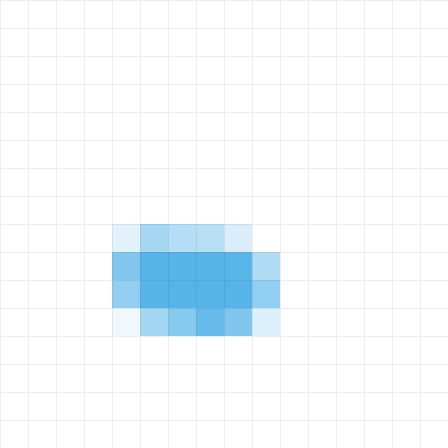
\includegraphics[width=0.85cm]{img/footprint16.png}};
\node[anchor=south, lbl] at (fp.north) {footprint $M$};
\node[anchor=north, note, align=center, inner sep=1.5pt] at (fp.south) {exact, from the\\[-1pt]aligned original};
\draw[<->, draw=ink] (map.east) -- node[above, font=\fontsize{5.8}{6}\selectfont, text=muted, inner sep=1.2pt]{BCE} node[below, font=\fontsize{5.8}{6}\selectfont, text=muted, inner sep=1.2pt]{+ Dice} (fp.west);
\node[thumb] (ovl) at (16.3,-0.55) {
\includegraphics[width=0.85cm]{img/ev_overlay.png}};
\node[anchor=south, lbl] at (ovl.north) {map on the crop};
\node[anchor=north, note, align=center, inner sep=1.5pt] at (ovl.south) {not read by\\[-1pt]the classifier};

\node[stage=ours, fill=white, dash pattern=on 2.2pt off 1.4pt, font=\smallfont, align=left, inner sep=2.6pt, anchor=west] (cons)
  at (10.85,-2.55) {$\mathcal{L}_\text{cons}=\lambda\,\bigl(z_f(x)-z_f(x_s)\bigr)^2$,\; $\lambda$\,=\,1, gradient through both sides\\[0.3pt]
  {\color{muted}$x_s$ has no class target; its map target is the footprint $M$ of $x$}};
\draw[tflow] (5.6,0 |- vit.south) |- node[pos=0.9, above, inner sep=1.5pt]{\shp{$z_f(x_s)$}} (cons.west);
\draw[tflow] (14.55,0 |- heads.south) -- (14.55,0.55) -- node[above, inner sep=1pt]{\shp{$z_f(x)$}} (15.12,0.55) -- (15.12,0 |- cons.north);
\node[anchor=north east, note, align=right] at ([yshift=-1pt]cons.south east) {dashed: training only (consistency variant)};
\end{tikzpicture}
\end{document}
